\section{The Approaches}\label{section:datasets}

\subsection{Method Selection}

why we chose these?

\subsection{Metrics and Evaluation}

For measuring the output of the selected methods, we have chosen to use \textbf{micro-averaged F1-score @k}. \footnote{More detailed information on this and other metrics and be found in \cite{sokolova_and_napalme_2009}.}

This measure was chosen due to the problem we wish to consider (namely, label ranking) and the way we want to average the results over a given dataset. In addition, this metric is commonly used in articles we have reviewed.

The F1-score (a particular case of the more general \textit{F-measure}, where $\beta$ equals 1) is widely used in information retrieval problems related to search or ranking of results; it is the harmonic mean of precision and recall, given by:

\begin{equation}
F_1 = 2 \cdot \frac{precision \cdot recall}{precision + recall} 
\end{equation}

which can be also written in terms of generic error metrics:

\begin{equation}
F_1 = \frac{2 \cdot true \ positive}{2 \cdot true \ positive + false \ negative + false \ positive} 
\end{equation}\\

With regards to \textit{micro-averaging}, it refers to the way we report results for the whole dataset, be it training or validation.

When \textit{macro-averaging} is used, equal weight is given to every class (label) in the dataset, which means that classes which occur only very rarely are given the same weight and very common classes when the full metrics over the dataset are calculated.

On the other hand, with \textit{micro-averaging}, the individual metrics (true positive, true negative, false positive and false negative) are aggregated over the whole dataset, which is preferable in cases (such as ours) where the dataset is highly unbalanced. \footnote{I.e. some labels appear much more often than others.}  

Finally, when metrics $@k$ are considered, it simply means that only the results up to the $k$-th position are taken into account when gathering the results:

\begin{equation}
F_1\ @k = \frac{2 \cdot true \ positive\ @k}{2 \cdot true \ positive\ @k + false \ negative\ @k + false \ positive\ @k} 
\end{equation}\\

This gives a more complete view of how the classifier works at different precision/recall levels, and can be easily visualized via graphical charts.


\subsection{TF-IDF Features, Binary Relevance and Linear SVM Classifier}



\subsubsection{Results on Dataset 1}



\subsubsection{Results on Dataset 2}

\begin{figure}[!h]
    \centering
    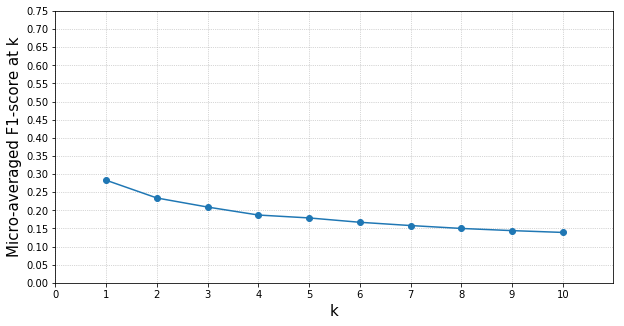
\includegraphics[width=\textwidth]{chapters/05_experiments/images/ovr-svm-movielens.png}
    \caption{Results on the Movielens Dataset, for k=1..10}
    \label{fig:ovr_svm_movielens}
\end{figure}

\subsubsection{Discussion}




\subsection{TF-IDF Features, k-Nearest Neighbours Classifier}

\subsubsection{Results on dataset 1}

\subsubsection{Results on Dataset 2}

\subsubsection{Discussion}


\subsection{MIMLSVM}

\subsubsection{Results on dataset 1}

\subsubsection{Results on Dataset 2}

\subsubsection{Discussion}



\subsection{Topic Distances}

In this approach, which has been suggested by \cite{choubey_2011},we first train a topic model on train set documents using Latent Dirichlet Allocation (LDA) (\cite{blei_2013}). Then, at query time, we calculate the topic distribution for the query document and also the single most similar train set document, as measured by the Kullback-Leibler Divergence (KL-Divergence, \cite{kullback_leibler_1951}) between the topic distributions of the documents. Finally, the tags used in the found document are used as suggestions for the unlabelled query document.

\subsubsection{Results on dataset 1}

\subsubsection{Results on Dataset 2}

\begin{figure}[!h]
    \centering
    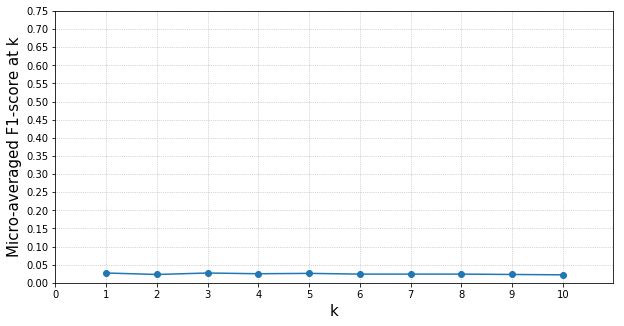
\includegraphics[width=\textwidth]{chapters/05_experiments/images/topic-distances-100d-movielens.png}
    \caption{Results on the Movielens Dataset, for k=1..10, using 100 components.}
    \label{fig:ovr_svm_movielens}
\end{figure}

\begin{figure}[!h]
    \centering
    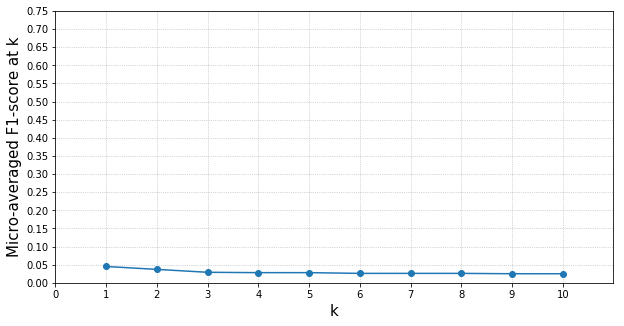
\includegraphics[width=\textwidth]{chapters/05_experiments/images/topic-distances-200d-movielens.png}
    \caption{Results on the Movielens Dataset, for k=1..10, using 200 components.}
    \label{fig:ovr_svm_movielens}
\end{figure}

\begin{figure}[!h]
    \centering
    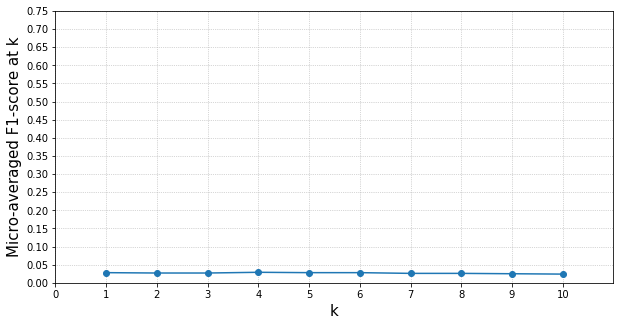
\includegraphics[width=\textwidth]{chapters/05_experiments/images/topic-distances-400d-movielens.png}
    \caption{Results on the Movielens Dataset, for k=1..10, using 400 components.}
    \label{fig:ovr_svm_movielens}
\end{figure}

\subsubsection{Discussion}

\subsection{Topic Words}

In this approach, also suggested by \cite{choubey_2011}, one trains an LDA topic model on documents in the train set. At test time, the topic distribution for each query document is calculated with the trained model. Then, the most representative words \footnote{Only words that are in the actual tag vocabulary are used.} for the most representative topic are suggested as tags for the query document.

\subsubsection{Results on dataset 1}

\subsubsection{Results on Dataset 2}

\begin{figure}[!h]
    \centering
    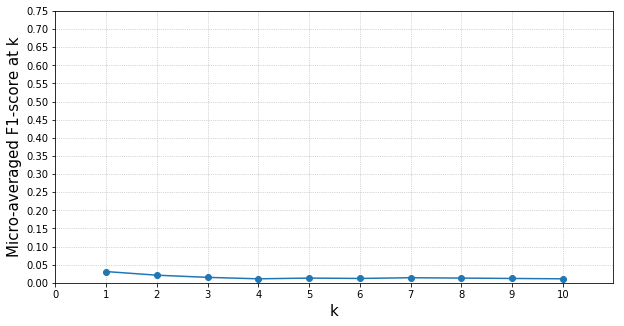
\includegraphics[width=\textwidth]{chapters/05_experiments/images/topic-words-100d-movielens.png}
    \caption{Results on the Movielens Dataset, for k=1..10, using 100 components.}
    \label{fig:ovr_svm_movielens}
\end{figure}

\begin{figure}[!h]
    \centering
    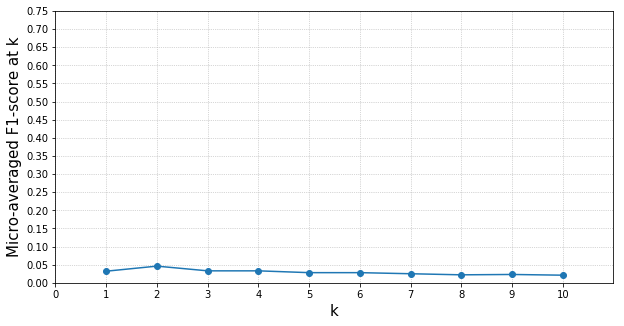
\includegraphics[width=\textwidth]{chapters/05_experiments/images/topic-words-200d-movielens.png}
    \caption{Results on the Movielens Dataset, for k=1..10, using 200 components.}
    \label{fig:ovr_svm_movielens}
\end{figure}

\begin{figure}[!h]
    \centering
    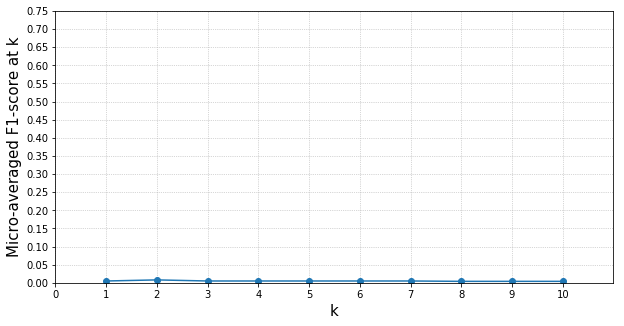
\includegraphics[width=\textwidth]{chapters/05_experiments/images/topic-words-400d-movielens.png}
    \caption{Results on the Movielens Dataset, for k=1..10, using 400 components.}
    \label{fig:ovr_svm_movielens}
\end{figure}

\subsubsection{Discussion}

\subsection{TF-IDF Features, MIMLSVM Classifier}

Multi-instance Learning \footnote{Also called \textit{Multiple-instance} Learning} is a technique (the name was first coined by \cite{dietterich_etal_1997}), whereby a an  instance in a traditional supervised learning problem is split into multiple so-called \textit{bags}.

\cite{shen_etal_2009} have applied multi-instance learning to the tag prediction problem, by first splitting the documents into segments using a well-known text segmentation algorithm called \textit{TextTiling} (\cite{hearst_1994}). In order to turn the multi-instance, multi-label problem into a regular single-instance, multi-label problem, the authors use \textit{k}-medoids clustering based on the Hausdorff distance (\cite{edgar_2008}). Finally, an SVM classifier is employed to classify the multi-label problem.


\subsection{Doc2Vec Document Features, Neural Network Classifier}

\subsubsection{Results on dataset 1}

\subsubsection{Results on Dataset 2}

\subsubsection{Discussion}


\subsection{Tags2Vec Document Features, Neural Network Classifier}

\subsubsection{Results on dataset 1}

\subsubsection{Results on Dataset 2}

\subsubsection{Discussion}

\subsection{Tags2Vec Document Features, Prototype Selection and Neural Network Classifier}

\subsubsection{Results on dataset 1}

\subsubsection{Results on Dataset 2}

\subsubsection{Discussion}

\subsection{Final Results}

